%!TEX root = ../documentation.tex

\chapter{Systemarchitektur}

Die Anwendung kann in drei große Komponenten zerlegt werden: Die Spiellogik, die Engine und den Levelgenerator.

Die Spiellogik steuert das Verhalten der einzelnen Elemente, die ein Teil unseres Spieles sind.

Die Engine bildet eine Abstraktionsschicht zwischen der Spiellogik und der Benutzereingabe sowie der Grafikausgabe. Durch den höheren Abstraktionsgrad kann die Spiellogik schneller und einfacher implementiert werden. Außerdem stellt die Engine in der Spiellogik mehrfach benötigte Funktionalitäten auf eine wiederverwendbaren Art und Weise zur Verfügung.

Der Levelgenerator hat die Aufgabe, zufallsbasiert die Level zu generieren, sodass diese bei jedem Spieldurchlauf anders wirken.

\begin{figure}[h]
	\centering
	% Graphic for TeX using PGF
% Title: /home/tobias/Documents/Studium/softwareengineering/organisation/documentations/softwareentwurf/uml-diagramms/Komponentendiagramm-high-level.dia
% Creator: Dia v0.97.2
% CreationDate: Sun Oct 25 21:55:41 2015
% For: tobias
% \usepackage{tikz}
% The following commands are not supported in PSTricks at present
% We define them conditionally, so when they are implemented,
% this pgf file will use them.
\ifx\du\undefined
  \newlength{\du}
\fi
\setlength{\du}{15\unitlength}
\begin{tikzpicture}
\pgftransformxscale{1.000000}
\pgftransformyscale{-1.000000}
\definecolor{dialinecolor}{rgb}{0.000000, 0.000000, 0.000000}
\pgfsetstrokecolor{dialinecolor}
\definecolor{dialinecolor}{rgb}{1.000000, 1.000000, 1.000000}
\pgfsetfillcolor{dialinecolor}
\definecolor{dialinecolor}{rgb}{1.000000, 1.000000, 1.000000}
\pgfsetfillcolor{dialinecolor}
\fill (15.850000\du,20.650000\du)--(15.850000\du,22.550000\du)--(22.847500\du,22.550000\du)--(22.847500\du,20.650000\du)--cycle;
\pgfsetlinewidth{0.100000\du}
\pgfsetdash{}{0pt}
\pgfsetdash{}{0pt}
\pgfsetmiterjoin
\definecolor{dialinecolor}{rgb}{0.000000, 0.000000, 0.000000}
\pgfsetstrokecolor{dialinecolor}
\draw (15.850000\du,20.650000\du)--(15.850000\du,22.550000\du)--(22.847500\du,22.550000\du)--(22.847500\du,20.650000\du)--cycle;
% setfont left to latex
\definecolor{dialinecolor}{rgb}{0.000000, 0.000000, 0.000000}
\pgfsetstrokecolor{dialinecolor}
\node at (19.348750\du,21.795000\du){Engine};
\definecolor{dialinecolor}{rgb}{1.000000, 1.000000, 1.000000}
\pgfsetfillcolor{dialinecolor}
\fill (19.550000\du,16.100000\du)--(19.550000\du,18.000000\du)--(26.573750\du,18.000000\du)--(26.573750\du,16.100000\du)--cycle;
\pgfsetlinewidth{0.100000\du}
\pgfsetdash{}{0pt}
\pgfsetdash{}{0pt}
\pgfsetmiterjoin
\definecolor{dialinecolor}{rgb}{0.000000, 0.000000, 0.000000}
\pgfsetstrokecolor{dialinecolor}
\draw (19.550000\du,16.100000\du)--(19.550000\du,18.000000\du)--(26.573750\du,18.000000\du)--(26.573750\du,16.100000\du)--cycle;
% setfont left to latex
\definecolor{dialinecolor}{rgb}{0.000000, 0.000000, 0.000000}
\pgfsetstrokecolor{dialinecolor}
\node at (23.061875\du,17.245000\du){Spiellogik};
\definecolor{dialinecolor}{rgb}{1.000000, 1.000000, 1.000000}
\pgfsetfillcolor{dialinecolor}
\fill (23.300000\du,20.650000\du)--(23.300000\du,22.550000\du)--(30.305000\du,22.550000\du)--(30.305000\du,20.650000\du)--cycle;
\pgfsetlinewidth{0.100000\du}
\pgfsetdash{}{0pt}
\pgfsetdash{}{0pt}
\pgfsetmiterjoin
\definecolor{dialinecolor}{rgb}{0.000000, 0.000000, 0.000000}
\pgfsetstrokecolor{dialinecolor}
\draw (23.300000\du,20.650000\du)--(23.300000\du,22.550000\du)--(30.305000\du,22.550000\du)--(30.305000\du,20.650000\du)--cycle;
% setfont left to latex
\definecolor{dialinecolor}{rgb}{0.000000, 0.000000, 0.000000}
\pgfsetstrokecolor{dialinecolor}
\node at (26.802500\du,21.795000\du){Levelgenerator};
\pgfsetlinewidth{0.100000\du}
\pgfsetdash{}{0pt}
\pgfsetdash{}{0pt}
\pgfsetbuttcap
{
\definecolor{dialinecolor}{rgb}{0.000000, 0.000000, 0.000000}
\pgfsetfillcolor{dialinecolor}
% was here!!!
\pgfsetarrowsend{stealth}
\definecolor{dialinecolor}{rgb}{0.000000, 0.000000, 0.000000}
\pgfsetstrokecolor{dialinecolor}
\draw (21.305937\du,18.000000\du)--(19.348750\du,20.650000\du);
}
\pgfsetlinewidth{0.100000\du}
\pgfsetdash{}{0pt}
\pgfsetdash{}{0pt}
\pgfsetbuttcap
{
\definecolor{dialinecolor}{rgb}{0.000000, 0.000000, 0.000000}
\pgfsetfillcolor{dialinecolor}
% was here!!!
\pgfsetarrowsend{stealth}
\definecolor{dialinecolor}{rgb}{0.000000, 0.000000, 0.000000}
\pgfsetstrokecolor{dialinecolor}
\draw (24.817813\du,18.000000\du)--(26.802500\du,20.650000\du);
}
% setfont left to latex
\definecolor{dialinecolor}{rgb}{0.000000, 0.000000, 0.000000}
\pgfsetstrokecolor{dialinecolor}
\node[anchor=west] at (26.250000\du,19.150000\du){Abhängig von};
% setfont left to latex
\definecolor{dialinecolor}{rgb}{0.000000, 0.000000, 0.000000}
\pgfsetstrokecolor{dialinecolor}
\node[anchor=west] at (15.550000\du,19.168687\du){Abhängig von};
\end{tikzpicture}

	\caption{Abhängigkeiten zwischen den drei highlevel-Komponenten der Software.}
\end{figure}

\section{Engine}

Die Anwendung besteht aus einer Sammlung von Szenen. Jede Szene repräsentiert eine Bildschirmseite, wie zum Beispiel das Pausenmenü, das Hauptmenü, oder ein Level. Zu jedem Zeitpunkt im Spiel ist genau eine Szene aktiv.

Jede Szene beinhaltet verschiedene Spielobjekte. Ein Spielobjekt ist ein atomarer Bestandteil einer Szene wie zum Beispiel ein Knopf in den Menüs, eine Wand, ein Stück Fußboden, ein NPC oder eine Pflanze.

Die wiederverwendbaren Funktionalitäten der Spielobjekte werden in Komponenten ausgelagert. Aus diesen können neue Spielobjekte schnell zusammengesetzt werden.

\begin{landscape}
	\begin{figure}
		\scalebox{0.75}{% Graphic for TeX using PGF
% Title: /home/tobias/Documents/Studium/softwareengineering/organisation/documentations/softwareentwurf/uml-diagramms/Classdiagram-structure-engine.dia
% Creator: Dia v0.97.2
% CreationDate: Sun Oct 18 15:37:55 2015
% For: tobias
% \usepackage{tikz}
% The following commands are not supported in PSTricks at present
% We define them conditionally, so when they are implemented,
% this pgf file will use them.
\ifx\du\undefined
  \newlength{\du}
\fi
\setlength{\du}{15\unitlength}
\begin{tikzpicture}
\pgftransformxscale{1.000000}
\pgftransformyscale{-1.000000}
\definecolor{dialinecolor}{rgb}{0.000000, 0.000000, 0.000000}
\pgfsetstrokecolor{dialinecolor}
\definecolor{dialinecolor}{rgb}{1.000000, 1.000000, 1.000000}
\pgfsetfillcolor{dialinecolor}
\pgfsetlinewidth{0.100000\du}
\pgfsetdash{}{0pt}
\definecolor{dialinecolor}{rgb}{1.000000, 1.000000, 1.000000}
\pgfsetfillcolor{dialinecolor}
\fill (15.424136\du,0.950000\du)--(15.424136\du,2.350000\du)--(30.554136\du,2.350000\du)--(30.554136\du,0.950000\du)--cycle;
\definecolor{dialinecolor}{rgb}{0.000000, 0.000000, 0.000000}
\pgfsetstrokecolor{dialinecolor}
\draw (15.424136\du,0.950000\du)--(15.424136\du,2.350000\du)--(30.554136\du,2.350000\du)--(30.554136\du,0.950000\du)--cycle;
% setfont left to latex
\definecolor{dialinecolor}{rgb}{0.000000, 0.000000, 0.000000}
\pgfsetstrokecolor{dialinecolor}
\node at (22.989136\du,1.900000\du){Game};
\definecolor{dialinecolor}{rgb}{1.000000, 1.000000, 1.000000}
\pgfsetfillcolor{dialinecolor}
\fill (15.424136\du,2.350000\du)--(15.424136\du,4.950000\du)--(30.554136\du,4.950000\du)--(30.554136\du,2.350000\du)--cycle;
\definecolor{dialinecolor}{rgb}{0.000000, 0.000000, 0.000000}
\pgfsetstrokecolor{dialinecolor}
\draw (15.424136\du,2.350000\du)--(15.424136\du,4.950000\du)--(30.554136\du,4.950000\du)--(30.554136\du,2.350000\du)--cycle;
% setfont left to latex
\definecolor{dialinecolor}{rgb}{0.000000, 0.000000, 0.000000}
\pgfsetstrokecolor{dialinecolor}
\node[anchor=west] at (15.574136\du,3.050000\du){+loadScene(scene:Scene): void};
% setfont left to latex
\definecolor{dialinecolor}{rgb}{0.000000, 0.000000, 0.000000}
\pgfsetstrokecolor{dialinecolor}
\node[anchor=west] at (15.574136\du,3.850000\du){+unloadCurrentScene(): void};
% setfont left to latex
\definecolor{dialinecolor}{rgb}{0.000000, 0.000000, 0.000000}
\pgfsetstrokecolor{dialinecolor}
\node[anchor=west] at (15.574136\du,4.650000\du){+startMainLoop(firstScene:Scene): void};
\pgfsetlinewidth{0.100000\du}
\pgfsetdash{}{0pt}
\definecolor{dialinecolor}{rgb}{1.000000, 1.000000, 1.000000}
\pgfsetfillcolor{dialinecolor}
\fill (15.231636\du,7.718324\du)--(15.231636\du,9.118324\du)--(30.746636\du,9.118324\du)--(30.746636\du,7.718324\du)--cycle;
\definecolor{dialinecolor}{rgb}{0.000000, 0.000000, 0.000000}
\pgfsetstrokecolor{dialinecolor}
\draw (15.231636\du,7.718324\du)--(15.231636\du,9.118324\du)--(30.746636\du,9.118324\du)--(30.746636\du,7.718324\du)--cycle;
% setfont left to latex
\definecolor{dialinecolor}{rgb}{0.000000, 0.000000, 0.000000}
\pgfsetstrokecolor{dialinecolor}
\node at (22.989136\du,8.668324\du){Scene};
\definecolor{dialinecolor}{rgb}{1.000000, 1.000000, 1.000000}
\pgfsetfillcolor{dialinecolor}
\fill (15.231636\du,9.118324\du)--(15.231636\du,10.918324\du)--(30.746636\du,10.918324\du)--(30.746636\du,9.118324\du)--cycle;
\definecolor{dialinecolor}{rgb}{0.000000, 0.000000, 0.000000}
\pgfsetstrokecolor{dialinecolor}
\draw (15.231636\du,9.118324\du)--(15.231636\du,10.918324\du)--(30.746636\du,10.918324\du)--(30.746636\du,9.118324\du)--cycle;
% setfont left to latex
\definecolor{dialinecolor}{rgb}{0.000000, 0.000000, 0.000000}
\pgfsetstrokecolor{dialinecolor}
\node[anchor=west] at (15.381636\du,9.818324\du){+registerGameObject(which:GameObject)};
% setfont left to latex
\definecolor{dialinecolor}{rgb}{0.000000, 0.000000, 0.000000}
\pgfsetstrokecolor{dialinecolor}
\node[anchor=west] at (15.381636\du,10.618324\du){+unregisterGameObject(which:GameObject)};
\pgfsetlinewidth{0.100000\du}
\pgfsetdash{}{0pt}
\definecolor{dialinecolor}{rgb}{1.000000, 1.000000, 1.000000}
\pgfsetfillcolor{dialinecolor}
\fill (19.989136\du,12.873073\du)--(19.989136\du,14.273073\du)--(25.989136\du,14.273073\du)--(25.989136\du,12.873073\du)--cycle;
\definecolor{dialinecolor}{rgb}{0.000000, 0.000000, 0.000000}
\pgfsetstrokecolor{dialinecolor}
\draw (19.989136\du,12.873073\du)--(19.989136\du,14.273073\du)--(25.989136\du,14.273073\du)--(25.989136\du,12.873073\du)--cycle;
% setfont left to latex
\definecolor{dialinecolor}{rgb}{0.000000, 0.000000, 0.000000}
\pgfsetstrokecolor{dialinecolor}
\node at (22.989136\du,13.823073\du){GameObject};
\pgfsetlinewidth{0.100000\du}
\pgfsetdash{}{0pt}
\definecolor{dialinecolor}{rgb}{1.000000, 1.000000, 1.000000}
\pgfsetfillcolor{dialinecolor}
\fill (30.700000\du,12.873073\du)--(30.700000\du,15.673073\du)--(45.830000\du,15.673073\du)--(45.830000\du,12.873073\du)--cycle;
\definecolor{dialinecolor}{rgb}{0.000000, 0.000000, 0.000000}
\pgfsetstrokecolor{dialinecolor}
\draw (30.700000\du,12.873073\du)--(30.700000\du,15.673073\du)--(45.830000\du,15.673073\du)--(45.830000\du,12.873073\du)--cycle;
% setfont left to latex
\definecolor{dialinecolor}{rgb}{0.000000, 0.000000, 0.000000}
\pgfsetstrokecolor{dialinecolor}
\node at (38.265000\du,13.823073\du){Position};
% setfont left to latex
\definecolor{dialinecolor}{rgb}{0.000000, 0.000000, 0.000000}
\pgfsetstrokecolor{dialinecolor}
\node at (38.265000\du,14.598073\du){An example for a};
\definecolor{dialinecolor}{rgb}{0.000000, 0.000000, 0.000000}
\pgfsetstrokecolor{dialinecolor}
\node at (38.265000\du,15.298073\du){component};
\definecolor{dialinecolor}{rgb}{1.000000, 1.000000, 1.000000}
\pgfsetfillcolor{dialinecolor}
\fill (30.700000\du,15.673073\du)--(30.700000\du,17.473073\du)--(45.830000\du,17.473073\du)--(45.830000\du,15.673073\du)--cycle;
\definecolor{dialinecolor}{rgb}{0.000000, 0.000000, 0.000000}
\pgfsetstrokecolor{dialinecolor}
\draw (30.700000\du,15.673073\du)--(30.700000\du,17.473073\du)--(45.830000\du,17.473073\du)--(45.830000\du,15.673073\du)--cycle;
% setfont left to latex
\definecolor{dialinecolor}{rgb}{0.000000, 0.000000, 0.000000}
\pgfsetstrokecolor{dialinecolor}
\node[anchor=west] at (30.850000\du,16.373073\du){+getPosition(): sf::vector2f};
% setfont left to latex
\definecolor{dialinecolor}{rgb}{0.000000, 0.000000, 0.000000}
\pgfsetstrokecolor{dialinecolor}
\node[anchor=west] at (30.850000\du,17.173073\du){+setPosition(value:sf::vector2f): void};
\pgfsetlinewidth{0.100000\du}
\pgfsetdash{}{0pt}
\definecolor{dialinecolor}{rgb}{1.000000, 1.000000, 1.000000}
\pgfsetfillcolor{dialinecolor}
\fill (46.555950\du,12.873073\du)--(46.555950\du,15.673073\du)--(60.145950\du,15.673073\du)--(60.145950\du,12.873073\du)--cycle;
\definecolor{dialinecolor}{rgb}{0.000000, 0.000000, 0.000000}
\pgfsetstrokecolor{dialinecolor}
\draw (46.555950\du,12.873073\du)--(46.555950\du,15.673073\du)--(60.145950\du,15.673073\du)--(60.145950\du,12.873073\du)--cycle;
% setfont left to latex
\definecolor{dialinecolor}{rgb}{0.000000, 0.000000, 0.000000}
\pgfsetstrokecolor{dialinecolor}
\node at (53.350950\du,13.823073\du){SoundEmitter};
% setfont left to latex
\definecolor{dialinecolor}{rgb}{0.000000, 0.000000, 0.000000}
\pgfsetstrokecolor{dialinecolor}
\node at (53.350950\du,14.598073\du){An example for a};
\definecolor{dialinecolor}{rgb}{0.000000, 0.000000, 0.000000}
\pgfsetstrokecolor{dialinecolor}
\node at (53.350950\du,15.298073\du){component};
\definecolor{dialinecolor}{rgb}{1.000000, 1.000000, 1.000000}
\pgfsetfillcolor{dialinecolor}
\fill (46.555950\du,15.673073\du)--(46.555950\du,16.673073\du)--(60.145950\du,16.673073\du)--(60.145950\du,15.673073\du)--cycle;
\definecolor{dialinecolor}{rgb}{0.000000, 0.000000, 0.000000}
\pgfsetstrokecolor{dialinecolor}
\draw (46.555950\du,15.673073\du)--(46.555950\du,16.673073\du)--(60.145950\du,16.673073\du)--(60.145950\du,15.673073\du)--cycle;
% setfont left to latex
\definecolor{dialinecolor}{rgb}{0.000000, 0.000000, 0.000000}
\pgfsetstrokecolor{dialinecolor}
\node[anchor=west] at (46.705950\du,16.373073\du){+play(soundfile:std::string): void};
\pgfsetlinewidth{0.100000\du}
\pgfsetdash{}{0pt}
\definecolor{dialinecolor}{rgb}{1.000000, 1.000000, 1.000000}
\pgfsetfillcolor{dialinecolor}
\fill (6.500000\du,20.050000\du)--(6.500000\du,21.450000\du)--(15.362500\du,21.450000\du)--(15.362500\du,20.050000\du)--cycle;
\definecolor{dialinecolor}{rgb}{0.000000, 0.000000, 0.000000}
\pgfsetstrokecolor{dialinecolor}
\draw (6.500000\du,20.050000\du)--(6.500000\du,21.450000\du)--(15.362500\du,21.450000\du)--(15.362500\du,20.050000\du)--cycle;
% setfont left to latex
\definecolor{dialinecolor}{rgb}{0.000000, 0.000000, 0.000000}
\pgfsetstrokecolor{dialinecolor}
\node at (10.931250\du,21.000000\du){ActualGameObject};
\pgfsetlinewidth{0.100000\du}
\pgfsetdash{}{0pt}
\pgfsetmiterjoin
\pgfsetbuttcap
{
\definecolor{dialinecolor}{rgb}{0.000000, 0.000000, 0.000000}
\pgfsetfillcolor{dialinecolor}
% was here!!!
\definecolor{dialinecolor}{rgb}{0.000000, 0.000000, 0.000000}
\pgfsetstrokecolor{dialinecolor}
\draw (19.989136\du,13.573073\du)--(10.931250\du,13.573073\du)--(10.931250\du,20.050000\du);
}
\definecolor{dialinecolor}{rgb}{0.000000, 0.000000, 0.000000}
\pgfsetstrokecolor{dialinecolor}
\draw (19.077333\du,13.573073\du)--(10.931250\du,13.573073\du)--(10.931250\du,20.050000\du);
\pgfsetmiterjoin
\definecolor{dialinecolor}{rgb}{1.000000, 1.000000, 1.000000}
\pgfsetfillcolor{dialinecolor}
\fill (19.077333\du,13.973073\du)--(19.877333\du,13.573073\du)--(19.077333\du,13.173073\du)--cycle;
\pgfsetlinewidth{0.100000\du}
\pgfsetdash{}{0pt}
\pgfsetmiterjoin
\definecolor{dialinecolor}{rgb}{0.000000, 0.000000, 0.000000}
\pgfsetstrokecolor{dialinecolor}
\draw (19.077333\du,13.973073\du)--(19.877333\du,13.573073\du)--(19.077333\du,13.173073\du)--cycle;
% setfont left to latex
\pgfsetlinewidth{0.100000\du}
\pgfsetdash{}{0pt}
\pgfsetmiterjoin
\pgfsetbuttcap
{
\definecolor{dialinecolor}{rgb}{0.000000, 0.000000, 0.000000}
\pgfsetfillcolor{dialinecolor}
% was here!!!
\definecolor{dialinecolor}{rgb}{0.000000, 0.000000, 0.000000}
\pgfsetstrokecolor{dialinecolor}
\draw (38.265000\du,17.473073\du)--(38.265000\du,20.750000\du)--(15.362500\du,20.750000\du);
}
\definecolor{dialinecolor}{rgb}{0.000000, 0.000000, 0.000000}
\pgfsetstrokecolor{dialinecolor}
\draw (38.265000\du,18.384876\du)--(38.265000\du,20.750000\du)--(15.362500\du,20.750000\du);
\pgfsetmiterjoin
\definecolor{dialinecolor}{rgb}{1.000000, 1.000000, 1.000000}
\pgfsetfillcolor{dialinecolor}
\fill (38.665000\du,18.384876\du)--(38.265000\du,17.584876\du)--(37.865000\du,18.384876\du)--cycle;
\pgfsetlinewidth{0.100000\du}
\pgfsetdash{}{0pt}
\pgfsetmiterjoin
\definecolor{dialinecolor}{rgb}{0.000000, 0.000000, 0.000000}
\pgfsetstrokecolor{dialinecolor}
\draw (38.665000\du,18.384876\du)--(38.265000\du,17.584876\du)--(37.865000\du,18.384876\du)--cycle;
% setfont left to latex
\pgfsetlinewidth{0.100000\du}
\pgfsetdash{}{0pt}
\pgfsetmiterjoin
\pgfsetbuttcap
{
\definecolor{dialinecolor}{rgb}{0.000000, 0.000000, 0.000000}
\pgfsetfillcolor{dialinecolor}
% was here!!!
\definecolor{dialinecolor}{rgb}{0.000000, 0.000000, 0.000000}
\pgfsetstrokecolor{dialinecolor}
\draw (53.350950\du,16.673073\du)--(53.350950\du,20.750000\du)--(15.362500\du,20.750000\du);
}
\definecolor{dialinecolor}{rgb}{0.000000, 0.000000, 0.000000}
\pgfsetstrokecolor{dialinecolor}
\draw (53.350950\du,17.584876\du)--(53.350950\du,20.750000\du)--(15.362500\du,20.750000\du);
\pgfsetmiterjoin
\definecolor{dialinecolor}{rgb}{1.000000, 1.000000, 1.000000}
\pgfsetfillcolor{dialinecolor}
\fill (53.750950\du,17.584876\du)--(53.350950\du,16.784876\du)--(52.950950\du,17.584876\du)--cycle;
\pgfsetlinewidth{0.100000\du}
\pgfsetdash{}{0pt}
\pgfsetmiterjoin
\definecolor{dialinecolor}{rgb}{0.000000, 0.000000, 0.000000}
\pgfsetstrokecolor{dialinecolor}
\draw (53.750950\du,17.584876\du)--(53.350950\du,16.784876\du)--(52.950950\du,17.584876\du)--cycle;
% setfont left to latex
\pgfsetlinewidth{0.100000\du}
\pgfsetdash{}{0pt}
\definecolor{dialinecolor}{rgb}{1.000000, 1.000000, 1.000000}
\pgfsetfillcolor{dialinecolor}
\fill (7.897500\du,11.100000\du)--(7.897500\du,12.500000\du)--(13.965000\du,12.500000\du)--(13.965000\du,11.100000\du)--cycle;
\definecolor{dialinecolor}{rgb}{0.000000, 0.000000, 0.000000}
\pgfsetstrokecolor{dialinecolor}
\draw (7.897500\du,11.100000\du)--(7.897500\du,12.500000\du)--(13.965000\du,12.500000\du)--(13.965000\du,11.100000\du)--cycle;
% setfont left to latex
\definecolor{dialinecolor}{rgb}{0.000000, 0.000000, 0.000000}
\pgfsetstrokecolor{dialinecolor}
\node at (10.931250\du,12.050000\du){ActualScene};
\pgfsetlinewidth{0.100000\du}
\pgfsetdash{}{0pt}
\pgfsetmiterjoin
\pgfsetbuttcap
{
\definecolor{dialinecolor}{rgb}{0.000000, 0.000000, 0.000000}
\pgfsetfillcolor{dialinecolor}
% was here!!!
\definecolor{dialinecolor}{rgb}{0.000000, 0.000000, 0.000000}
\pgfsetstrokecolor{dialinecolor}
\draw (15.231636\du,8.418324\du)--(10.931250\du,8.418324\du)--(10.931250\du,11.100000\du);
}
\definecolor{dialinecolor}{rgb}{0.000000, 0.000000, 0.000000}
\pgfsetstrokecolor{dialinecolor}
\draw (14.319833\du,8.418324\du)--(10.931250\du,8.418324\du)--(10.931250\du,11.100000\du);
\pgfsetmiterjoin
\definecolor{dialinecolor}{rgb}{1.000000, 1.000000, 1.000000}
\pgfsetfillcolor{dialinecolor}
\fill (14.319833\du,8.818324\du)--(15.119833\du,8.418324\du)--(14.319833\du,8.018324\du)--cycle;
\pgfsetlinewidth{0.100000\du}
\pgfsetdash{}{0pt}
\pgfsetmiterjoin
\definecolor{dialinecolor}{rgb}{0.000000, 0.000000, 0.000000}
\pgfsetstrokecolor{dialinecolor}
\draw (14.319833\du,8.818324\du)--(15.119833\du,8.418324\du)--(14.319833\du,8.018324\du)--cycle;
% setfont left to latex
\pgfsetlinewidth{0.100000\du}
\pgfsetdash{}{0pt}
\pgfsetmiterjoin
\pgfsetbuttcap
{
\definecolor{dialinecolor}{rgb}{0.000000, 0.000000, 0.000000}
\pgfsetfillcolor{dialinecolor}
% was here!!!
\definecolor{dialinecolor}{rgb}{0.000000, 0.000000, 0.000000}
\pgfsetstrokecolor{dialinecolor}
\draw (22.989136\du,5.000250\du)--(22.989136\du,5.750250\du)--(22.989136\du,7.617921\du)--(22.989136\du,7.667921\du);
}
\definecolor{dialinecolor}{rgb}{0.000000, 0.000000, 0.000000}
\pgfsetstrokecolor{dialinecolor}
\draw (22.989136\du,6.258829\du)--(22.989136\du,5.750250\du)--(22.989136\du,7.617921\du)--(22.989136\du,7.667921\du);
\pgfsetdash{}{0pt}
\pgfsetmiterjoin
\pgfsetbuttcap
\definecolor{dialinecolor}{rgb}{1.000000, 1.000000, 1.000000}
\pgfsetfillcolor{dialinecolor}
\fill (22.989136\du,5.000250\du)--(23.229136\du,5.700250\du)--(22.989136\du,6.400250\du)--(22.749136\du,5.700250\du)--cycle;
\pgfsetlinewidth{0.100000\du}
\pgfsetdash{}{0pt}
\pgfsetmiterjoin
\pgfsetbuttcap
\definecolor{dialinecolor}{rgb}{0.000000, 0.000000, 0.000000}
\pgfsetstrokecolor{dialinecolor}
\draw (22.989136\du,5.000250\du)--(23.229136\du,5.700250\du)--(22.989136\du,6.400250\du)--(22.749136\du,5.700250\du)--cycle;
% setfont left to latex
\pgfsetlinewidth{0.100000\du}
\pgfsetdash{}{0pt}
\pgfsetmiterjoin
\pgfsetbuttcap
{
\definecolor{dialinecolor}{rgb}{0.000000, 0.000000, 0.000000}
\pgfsetfillcolor{dialinecolor}
% was here!!!
\definecolor{dialinecolor}{rgb}{0.000000, 0.000000, 0.000000}
\pgfsetstrokecolor{dialinecolor}
\draw (22.989136\du,10.968727\du)--(22.989136\du,11.718727\du)--(22.989136\du,12.772707\du)--(22.989136\du,12.822707\du);
}
\definecolor{dialinecolor}{rgb}{0.000000, 0.000000, 0.000000}
\pgfsetstrokecolor{dialinecolor}
\draw (22.989136\du,12.227306\du)--(22.989136\du,11.718727\du)--(22.989136\du,12.772707\du)--(22.989136\du,12.822707\du);
\pgfsetdash{}{0pt}
\pgfsetmiterjoin
\pgfsetbuttcap
\definecolor{dialinecolor}{rgb}{1.000000, 1.000000, 1.000000}
\pgfsetfillcolor{dialinecolor}
\fill (22.989136\du,10.968727\du)--(23.229136\du,11.668727\du)--(22.989136\du,12.368727\du)--(22.749136\du,11.668727\du)--cycle;
\pgfsetlinewidth{0.100000\du}
\pgfsetdash{}{0pt}
\pgfsetmiterjoin
\pgfsetbuttcap
\definecolor{dialinecolor}{rgb}{0.000000, 0.000000, 0.000000}
\pgfsetstrokecolor{dialinecolor}
\draw (22.989136\du,10.968727\du)--(23.229136\du,11.668727\du)--(22.989136\du,12.368727\du)--(22.749136\du,11.668727\du)--cycle;
% setfont left to latex
\end{tikzpicture}
}
		\caption{Zusammenfassendes Klassendiagramm der Spielarchitektur}
	\end{figure}
\end{landscape}

	\subsection{Spielobjekte}
	
	Jeder Spielobjekt-Typ wird als eigene Klasse umgesetzt. Die Spielobjekte erben alle von einer gemeinsamen Vaterklasse \enquote{GameObject}.

		\subsubsection{Komponentensystem}

		Viele Funktionalitäten wiederholen sich bei den einzelnen Spielobjekten. Es werden jedoch nicht immer alle Funktionalitäten in jedem Spielobjekt benötigt. Dabei ist es wichtig, dass Funktionalitäten, die in einem Spielobjekt nicht benötigt wird, auch tatsächlich inaktiv oder gar nicht erst vorhanden sind. Bei einigen Funktionalitäten, wie beispielsweise der Kollisionserkennung, hat es nämlich starke negative Auswirkungen auf die Performance, wenn sie auf zu vielen Spielobjekten angewendet werden. Die unterschiedlichen Kombinationen dieser Funktionalitäten lassen sich jedoch nicht immer durch einen \enquote{klassischen Vererbungsbaum} ausdrücken.

		Die wiederverwendbaren Funktionalitäten von Spielobjekten werden in Komponenten ausgelagert. Jede Komponente wird als Klasse umgesetzt, die später ein Teil des Spielobjekts ist. Über virtuelle Mehrfachvererbung werden Abhängigkeiten zwischen den Komponenten ausgedrückt und Komponenten zu GameObject-Klassen hinzugefügt.
	
		\begin{figure}[h]
			\centering
			% Graphic for TeX using PGF
% Title: /home/tobias/Documents/Studium/softwareengineering/organisation/documentations/softwareentwurf/uml-diagramms/Classdiagramm-components-diamond.dia
% Creator: Dia v0.97.2
% CreationDate: Sun Oct 18 15:39:25 2015
% For: tobias
% \usepackage{tikz}
% The following commands are not supported in PSTricks at present
% We define them conditionally, so when they are implemented,
% this pgf file will use them.
\ifx\du\undefined
  \newlength{\du}
\fi
\setlength{\du}{15\unitlength}
\begin{tikzpicture}
\pgftransformxscale{1.000000}
\pgftransformyscale{-1.000000}
\definecolor{dialinecolor}{rgb}{0.000000, 0.000000, 0.000000}
\pgfsetstrokecolor{dialinecolor}
\definecolor{dialinecolor}{rgb}{1.000000, 1.000000, 1.000000}
\pgfsetfillcolor{dialinecolor}
\pgfsetlinewidth{0.100000\du}
\pgfsetdash{}{0pt}
\definecolor{dialinecolor}{rgb}{1.000000, 1.000000, 1.000000}
\pgfsetfillcolor{dialinecolor}
\fill (20.165000\du,19.750000\du)--(20.165000\du,21.150000\du)--(29.027500\du,21.150000\du)--(29.027500\du,19.750000\du)--cycle;
\definecolor{dialinecolor}{rgb}{0.000000, 0.000000, 0.000000}
\pgfsetstrokecolor{dialinecolor}
\draw (20.165000\du,19.750000\du)--(20.165000\du,21.150000\du)--(29.027500\du,21.150000\du)--(29.027500\du,19.750000\du)--cycle;
% setfont left to latex
\definecolor{dialinecolor}{rgb}{0.000000, 0.000000, 0.000000}
\pgfsetstrokecolor{dialinecolor}
\node at (24.596250\du,20.700000\du){ActualGameObject};
\pgfsetlinewidth{0.100000\du}
\pgfsetdash{}{0pt}
\definecolor{dialinecolor}{rgb}{1.000000, 1.000000, 1.000000}
\pgfsetfillcolor{dialinecolor}
\fill (21.596250\du,15.000000\du)--(21.596250\du,16.400000\du)--(27.596250\du,16.400000\du)--(27.596250\du,15.000000\du)--cycle;
\definecolor{dialinecolor}{rgb}{0.000000, 0.000000, 0.000000}
\pgfsetstrokecolor{dialinecolor}
\draw (21.596250\du,15.000000\du)--(21.596250\du,16.400000\du)--(27.596250\du,16.400000\du)--(27.596250\du,15.000000\du)--cycle;
% setfont left to latex
\definecolor{dialinecolor}{rgb}{0.000000, 0.000000, 0.000000}
\pgfsetstrokecolor{dialinecolor}
\node at (24.596250\du,15.950000\du){GameObject};
\pgfsetlinewidth{0.100000\du}
\pgfsetdash{}{0pt}
\definecolor{dialinecolor}{rgb}{1.000000, 1.000000, 1.000000}
\pgfsetfillcolor{dialinecolor}
\fill (33.900000\du,10.200000\du)--(33.900000\du,11.600000\du)--(38.065000\du,11.600000\du)--(38.065000\du,10.200000\du)--cycle;
\definecolor{dialinecolor}{rgb}{0.000000, 0.000000, 0.000000}
\pgfsetstrokecolor{dialinecolor}
\draw (33.900000\du,10.200000\du)--(33.900000\du,11.600000\du)--(38.065000\du,11.600000\du)--(38.065000\du,10.200000\du)--cycle;
% setfont left to latex
\definecolor{dialinecolor}{rgb}{0.000000, 0.000000, 0.000000}
\pgfsetstrokecolor{dialinecolor}
\node at (35.982500\du,11.150000\du){Position};
\pgfsetlinewidth{0.100000\du}
\pgfsetdash{}{0pt}
\definecolor{dialinecolor}{rgb}{1.000000, 1.000000, 1.000000}
\pgfsetfillcolor{dialinecolor}
\fill (32.015000\du,16.000000\du)--(32.015000\du,17.400000\du)--(35.320000\du,17.400000\du)--(35.320000\du,16.000000\du)--cycle;
\definecolor{dialinecolor}{rgb}{0.000000, 0.000000, 0.000000}
\pgfsetstrokecolor{dialinecolor}
\draw (32.015000\du,16.000000\du)--(32.015000\du,17.400000\du)--(35.320000\du,17.400000\du)--(35.320000\du,16.000000\du)--cycle;
% setfont left to latex
\definecolor{dialinecolor}{rgb}{0.000000, 0.000000, 0.000000}
\pgfsetstrokecolor{dialinecolor}
\node at (33.667500\du,16.950000\du){Speed};
\pgfsetlinewidth{0.100000\du}
\pgfsetdash{}{0pt}
\definecolor{dialinecolor}{rgb}{1.000000, 1.000000, 1.000000}
\pgfsetfillcolor{dialinecolor}
\fill (37.015000\du,16.000000\du)--(37.015000\du,17.400000\du)--(40.257500\du,17.400000\du)--(40.257500\du,16.000000\du)--cycle;
\definecolor{dialinecolor}{rgb}{0.000000, 0.000000, 0.000000}
\pgfsetstrokecolor{dialinecolor}
\draw (37.015000\du,16.000000\du)--(37.015000\du,17.400000\du)--(40.257500\du,17.400000\du)--(40.257500\du,16.000000\du)--cycle;
% setfont left to latex
\definecolor{dialinecolor}{rgb}{0.000000, 0.000000, 0.000000}
\pgfsetstrokecolor{dialinecolor}
\node at (38.636250\du,16.950000\du){Sprite};
\pgfsetlinewidth{0.100000\du}
\pgfsetdash{}{0pt}
\pgfsetmiterjoin
\pgfsetbuttcap
{
\definecolor{dialinecolor}{rgb}{0.000000, 0.000000, 0.000000}
\pgfsetfillcolor{dialinecolor}
% was here!!!
\definecolor{dialinecolor}{rgb}{0.000000, 0.000000, 0.000000}
\pgfsetstrokecolor{dialinecolor}
\draw (35.982500\du,11.650366\du)--(35.982500\du,14.200000\du)--(33.667500\du,14.200000\du)--(33.667500\du,15.949634\du);
}
\definecolor{dialinecolor}{rgb}{0.000000, 0.000000, 0.000000}
\pgfsetstrokecolor{dialinecolor}
\draw (35.982500\du,12.562170\du)--(35.982500\du,14.200000\du)--(33.667500\du,14.200000\du)--(33.667500\du,15.949634\du);
\pgfsetmiterjoin
\definecolor{dialinecolor}{rgb}{1.000000, 1.000000, 1.000000}
\pgfsetfillcolor{dialinecolor}
\fill (36.382500\du,12.562170\du)--(35.982500\du,11.762170\du)--(35.582500\du,12.562170\du)--cycle;
\pgfsetlinewidth{0.100000\du}
\pgfsetdash{}{0pt}
\pgfsetmiterjoin
\definecolor{dialinecolor}{rgb}{0.000000, 0.000000, 0.000000}
\pgfsetstrokecolor{dialinecolor}
\draw (36.382500\du,12.562170\du)--(35.982500\du,11.762170\du)--(35.582500\du,12.562170\du)--cycle;
% setfont left to latex
\pgfsetlinewidth{0.100000\du}
\pgfsetdash{}{0pt}
\pgfsetmiterjoin
\pgfsetbuttcap
{
\definecolor{dialinecolor}{rgb}{0.000000, 0.000000, 0.000000}
\pgfsetfillcolor{dialinecolor}
% was here!!!
\definecolor{dialinecolor}{rgb}{0.000000, 0.000000, 0.000000}
\pgfsetstrokecolor{dialinecolor}
\draw (35.982500\du,11.650366\du)--(35.982500\du,14.200000\du)--(38.636250\du,14.200000\du)--(38.636250\du,15.949634\du);
}
\definecolor{dialinecolor}{rgb}{0.000000, 0.000000, 0.000000}
\pgfsetstrokecolor{dialinecolor}
\draw (35.982500\du,12.562170\du)--(35.982500\du,14.200000\du)--(38.636250\du,14.200000\du)--(38.636250\du,15.949634\du);
\pgfsetmiterjoin
\definecolor{dialinecolor}{rgb}{1.000000, 1.000000, 1.000000}
\pgfsetfillcolor{dialinecolor}
\fill (36.382500\du,12.562170\du)--(35.982500\du,11.762170\du)--(35.582500\du,12.562170\du)--cycle;
\pgfsetlinewidth{0.100000\du}
\pgfsetdash{}{0pt}
\pgfsetmiterjoin
\definecolor{dialinecolor}{rgb}{0.000000, 0.000000, 0.000000}
\pgfsetstrokecolor{dialinecolor}
\draw (36.382500\du,12.562170\du)--(35.982500\du,11.762170\du)--(35.582500\du,12.562170\du)--cycle;
% setfont left to latex
\pgfsetlinewidth{0.100000\du}
\pgfsetdash{}{0pt}
\pgfsetmiterjoin
\pgfsetbuttcap
{
\definecolor{dialinecolor}{rgb}{0.000000, 0.000000, 0.000000}
\pgfsetfillcolor{dialinecolor}
% was here!!!
\definecolor{dialinecolor}{rgb}{0.000000, 0.000000, 0.000000}
\pgfsetstrokecolor{dialinecolor}
\draw (33.667500\du,17.400000\du)--(33.667500\du,20.450000\du)--(29.027500\du,20.450000\du);
}
\definecolor{dialinecolor}{rgb}{0.000000, 0.000000, 0.000000}
\pgfsetstrokecolor{dialinecolor}
\draw (33.667500\du,18.311803\du)--(33.667500\du,20.450000\du)--(29.027500\du,20.450000\du);
\pgfsetmiterjoin
\definecolor{dialinecolor}{rgb}{1.000000, 1.000000, 1.000000}
\pgfsetfillcolor{dialinecolor}
\fill (34.067500\du,18.311803\du)--(33.667500\du,17.511803\du)--(33.267500\du,18.311803\du)--cycle;
\pgfsetlinewidth{0.100000\du}
\pgfsetdash{}{0pt}
\pgfsetmiterjoin
\definecolor{dialinecolor}{rgb}{0.000000, 0.000000, 0.000000}
\pgfsetstrokecolor{dialinecolor}
\draw (34.067500\du,18.311803\du)--(33.667500\du,17.511803\du)--(33.267500\du,18.311803\du)--cycle;
% setfont left to latex
\pgfsetlinewidth{0.100000\du}
\pgfsetdash{}{0pt}
\pgfsetmiterjoin
\pgfsetbuttcap
{
\definecolor{dialinecolor}{rgb}{0.000000, 0.000000, 0.000000}
\pgfsetfillcolor{dialinecolor}
% was here!!!
\definecolor{dialinecolor}{rgb}{0.000000, 0.000000, 0.000000}
\pgfsetstrokecolor{dialinecolor}
\draw (38.636250\du,17.400000\du)--(38.636250\du,20.450000\du)--(29.027500\du,20.450000\du);
}
\definecolor{dialinecolor}{rgb}{0.000000, 0.000000, 0.000000}
\pgfsetstrokecolor{dialinecolor}
\draw (38.636250\du,18.311803\du)--(38.636250\du,20.450000\du)--(29.027500\du,20.450000\du);
\pgfsetmiterjoin
\definecolor{dialinecolor}{rgb}{1.000000, 1.000000, 1.000000}
\pgfsetfillcolor{dialinecolor}
\fill (39.036250\du,18.311803\du)--(38.636250\du,17.511803\du)--(38.236250\du,18.311803\du)--cycle;
\pgfsetlinewidth{0.100000\du}
\pgfsetdash{}{0pt}
\pgfsetmiterjoin
\definecolor{dialinecolor}{rgb}{0.000000, 0.000000, 0.000000}
\pgfsetstrokecolor{dialinecolor}
\draw (39.036250\du,18.311803\du)--(38.636250\du,17.511803\du)--(38.236250\du,18.311803\du)--cycle;
% setfont left to latex
\pgfsetlinewidth{0.100000\du}
\pgfsetdash{}{0pt}
\pgfsetmiterjoin
\pgfsetbuttcap
{
\definecolor{dialinecolor}{rgb}{0.000000, 0.000000, 0.000000}
\pgfsetfillcolor{dialinecolor}
% was here!!!
\definecolor{dialinecolor}{rgb}{0.000000, 0.000000, 0.000000}
\pgfsetstrokecolor{dialinecolor}
\draw (24.596250\du,16.450366\du)--(24.596250\du,17.300366\du)--(24.596250\du,19.649634\du)--(24.596250\du,19.699634\du);
}
\definecolor{dialinecolor}{rgb}{0.000000, 0.000000, 0.000000}
\pgfsetstrokecolor{dialinecolor}
\draw (24.596250\du,17.362170\du)--(24.596250\du,17.300366\du)--(24.596250\du,19.649634\du)--(24.596250\du,19.699634\du);
\pgfsetmiterjoin
\definecolor{dialinecolor}{rgb}{1.000000, 1.000000, 1.000000}
\pgfsetfillcolor{dialinecolor}
\fill (24.996250\du,17.362170\du)--(24.596250\du,16.562170\du)--(24.196250\du,17.362170\du)--cycle;
\pgfsetlinewidth{0.100000\du}
\pgfsetdash{}{0pt}
\pgfsetmiterjoin
\definecolor{dialinecolor}{rgb}{0.000000, 0.000000, 0.000000}
\pgfsetstrokecolor{dialinecolor}
\draw (24.996250\du,17.362170\du)--(24.596250\du,16.562170\du)--(24.196250\du,17.362170\du)--cycle;
% setfont left to latex
% setfont left to latex
\definecolor{dialinecolor}{rgb}{0.000000, 0.000000, 0.000000}
\pgfsetstrokecolor{dialinecolor}
\node[anchor=west] at (39.050000\du,15.000000\du){<<virtual>>};
% setfont left to latex
\definecolor{dialinecolor}{rgb}{0.000000, 0.000000, 0.000000}
\pgfsetstrokecolor{dialinecolor}
\node[anchor=west] at (29.065000\du,14.995000\du){<<virtual>>};
% setfont left to latex
\definecolor{dialinecolor}{rgb}{0.000000, 0.000000, 0.000000}
\pgfsetstrokecolor{dialinecolor}
\node[anchor=west] at (29.045000\du,18.995000\du){<<virtual>>};
% setfont left to latex
\definecolor{dialinecolor}{rgb}{0.000000, 0.000000, 0.000000}
\pgfsetstrokecolor{dialinecolor}
\node[anchor=west] at (39.010000\du,18.995000\du){<<virtual>>};
\end{tikzpicture}

			\caption{Komponentensystem}
			\medskip
			\small
			Durch die virtuelle Mehrfachvererbung wird das Diamond-Problem gelöst. (\url{https://de.wikipedia.org/wiki/Diamond-Problem})
		\end{figure}

		\subsubsection{Kommunikation zwischen Komponenten}

		Häufig ist es notwendig, dass Komponenten, die voneinander abhängig sind, sich untereinander über bestimmte Ereignisse informieren. So könnte beispielsweise die Kollisionserkennungs-Komponente von der Positions-Komponente benachrichtigt werden, dass sich die Position des Spielobjektes geändert hat. Da allerdings eventuell noch weitere Komponenten über die Änderung der Position benachrichtigt werden müssen, ist eine einfache Umsetzung über eine virtuelle Funktion nicht möglich. Stattdessen wird das Publish-Subscribe-Pattern zur Kommunikation zwischen den Komponenten verwendet.
		
		Komponenten können ein \enquote{Publisher}-Objekt anbieten, um bestimmte Ereignisse mit anderen Komponenten zu \enquote{teilen}. Die anderen Komponenten können sich bei dem Publisher-Objekt mit einem Funktionspointer registrieren. Wenn die anbietende Komponente das Ereignis auslöst, werden alle registrierten Funktionspointer aufgerufen und so die anderen Komponenten benachrichtigt.
		
		%
		% TODO: Hier evtl Klassendiagramm Publish-Subscribe
		%

		\subsubsection{Die wichtigsten Komponenten}

		Hier eine Übersicht über die Komponenten, die für die Umsetzung des Projektes essentiell sind:

		\begin{longtable}{|l|p{3cm}|p{6cm}|p{3cm}|}
			\hline
			\textbf{ID} 
				& \textbf{Name} 
					& \textbf{Beschreibung} 
						& \textbf{Abhängig von}
			\\ \hline

			C-10 	& Update 
					& Erlaubt dem Spielobjekt, während der Update-Phase, also immer vor dem Zeichnen eines neuen Bildes, eine Aktion durchzuführen. Dies wird durch einen Publisher, der von dieser Komponente bereitgestellt wird, ermöglicht.
						& -

			\\ \hline

			C-20 	& Position 
					& Gibt dem Spielobjekt eine Position in Form einer X/Y-Koordinate.
						& -
			\\ \hline

			C-30 	& Speed 
					& Gibt dem Spielobjekt eine Geschwindigkeit in Form eines Richtungsvektors. Die Position des Spielobjektes wird entsprechend animiert.
						& Update, Position
			\\ \hline

			C-40 	& Drawable 
					& Ermöglicht es dem Spielobjekt, eine grafische Repräsentation jeglicher Art (Bitmapgrafik, Text, Rechteck, ...)  zu haben.
						& Position 
			\\ \hline

			C-50 	& Text 	
					& Weist dem Spielobjekt einen Text, der angezeigt werden soll, zu.
						& Drawable
			\\ \hline

			C-60 	& Sprite 
					& Weist dem Spielobjekt eine (Bitmap-)Grafik zu.
						& Drawable 
			\\ \hline 

			C-70 	& Animation
					& Weist dem Spielobjekt eine ständig wechselnde Grafik zu. So werden \enquote{Daumenkino-Animationen} möglich.
						& Sprite, Update 

			\\ \hline 

			C-80 	& Solide
					& Fügt dem Spielobjekt eine rechteckige Fläche hinzu, die zur Kollisionserkennung genutzt wird. Diese Fläche wird relativ zur eigenen Position angegeben.
						& Position
			\\ \hline

			C-90 	& CollisionDetector
					& Benachrichtigt das Spielobjekt, wenn sich die eigene Kollisionsfläche aus der Solide-Komponente mit einer anderen Kollisionsfläche überschneidet.
						& Solide
			\\ \hline

			C-100 	& CollisionResolver
					& Wenn das Spielobjekt mit einem anderen Spielobjekt kollidiert, löst diese Komponente die Kollision automatisch auf, indem sie die Position so anpasst, dass sich die beiden Objekte nicht mehr überschneiden.
						& CollisionDetector, Position
			\\ \hline

			C-110 	& MouseInput 
					& Ermöglicht dem Spielobjekt durch das Bereitstellen entsprechender Publisher-Objekte, auf Mauseingaben zu reagieren.
						& -

			\\ \hline

			C-120 	& KeyboardInput 
					& Ermöglicht dem Spielobjekt durch das Bereitstellen entsprechender Publisher-Objekte, auf Tastatureingaben zu reagieren.
						& -
			\\ \hline

			C-130 	& MessageSender <MessageType> 
					& (Klassentemplate) Erlaubt es dem Spielobjekt, Nachrichten an andere Spielobjekte zu verschicken. Eine Nachricht ist ein Objekt vom Typ MessageType.  Die Spielobjekte, die die Nachricht erhalten, können durch eine maximale Entfernung beschränkt werden. Außerdem ist es möglich, die Nachricht nur an das nächste Spielobjekt zu senden, das die Nachricht empfangen kann. So ist eine Kommunikation zwischen Spielobjekten möglich, ohne dass große Abhängigkeiten zwischen diesen entstehen.
						& Position
			\\ \hline
			
			C-140 	& MessageReceiver <MessageType> 
					& Das Gegenstück zum MessageSender.
						& Position
			\\ \hline
		\end{longtable}

	\subsection{Szene}
	
		Jede Szene im Spiel wird mittels einer eigenen Klasse umgesetzt, die von der abstrakten Klasse \enquote{Scene} erbt.

		\subsubsection{Verwaltung der Spielobjekte}
		
		Die initialen Spielobjekte werden im Konstruktor von der (abgeleiteten) Szenen-Klasse erzeugt. Alle Spielobjekte werden in einem gemeinsamen Array verwaltet.

		Spielobjekte, die Komponenten beinhalten, die Interaktionen mit der Szene erfordern, werden durch diese noch einmal extra bei der Szene registriert. Diese kann die Komponenten-Registrierungen dann getrennt voneinander verwalten.
		
		Ein Beispiel dafür is die Update-Komponente. Sie muss sich bei der Szene für den Erhalt der Update-Ereignisse registrieren. So ist die Szene immer im Besitz einer vollständigen Liste aller Spielobjekte mit Update-Komponente. Nur an diese Spielobjekte muss die Scene das Update-Event weitergeben.

		Die Verwaltung der Komponenten-Registrierungen erfolgt nicht generalisiert, sondern je nach Komponente individuell. So können immer die passenden Datenstrukturen verwendet werden. Bei der Update-Komponente ist es zum Beispiel am sinnvollsten, diese in einem einfachen Array zu verwalten. Bei den Komponenten zur Kollisionserkennung macht dagegen eine Verwaltung in einem QuadTree mehr Sinn.

		\subsubsection{Ebenen}

		Die Szene steuert auch den Zeichenprozess aller Spielobjekte. Dabei stellt sie 5 verschiedene Ebenen zur Verfügung:

		\begin{itemize}
			\item \textbf{Ebene 0}: Fußboden, Sonstiger Hintergrund
			\item \textbf{Ebene 1}: Schatten
			\item \textbf{Ebene 2}: Wände, Gegenstände, NPCs und der Spielcharakter. Die Spielobjekte dieser Ebene werden vor dem Zeichnen nach der Y-Koordinate sortiert, damit sich die Gegenstände korrekt überlappen.
			\item \textbf{Ebene 3}: Alles, wo der Spieler drunter hindurch gehen kann. Wolken, Baumkronen
			\item \textbf{Ebene 4}: Knöpfe, Punkteanzeigen, sonstige Steuerelemente, die als Overlay unabhängig vom gezeigten Kartenausschnitt immer gleich angezeigt werden.
		\end{itemize}

	\subsection{Game}
		Es existiert eine Klasse \enquote{Game}. Dies ist die Hauptklasse, in der die gestarteten Szenen und alle Ressourcen, die global verfügbar sein müssen, verwaltet werden. Ist die Hauptschleife des Spiels in dieser Klasse implementiert.

		\subsubsection{Organisation der Szenen}
		
		Neue Szenen können über eine Methode gestartet werden, der die entsprechende Szene als Parameter übergeben wird.

		Alle gestarteten Szenen werden auf einem Stack verwaltet. Die oberste Szene ist dabei die aktive Szene, alle anderen Szenen sind pausiert. Wird eine neue Szene gestartet, so wird diese auf den Stack geschoben und ersetzt so die vorherige aktive Szene. Wird die aktive Szene beendet, so wird sie wieder vom Stack entfernt. Dadurch wird die vorherige Szene wieder aktiv. So ist es einfach, (Pausen-)Menüs oder Anzeigen zu erstellen, bei denen der Benutzer nach dem Schließen wieder zurück zum Spiel kommt.

		\subsubsection{Globale Ressourcen}
		Die globalen Ressourcen, die in der Game-Klasse verwaltet werden sind insbesondere:

		\begin{enumerate}
			\item Das Hauptfenster
			\item Die Texturen
		\end{enumerate}

		\subsubsection{Hauptschleife}
		Nachdem die grundlegenden Bestandteile der Applikation initialisiert wurden, wird die Hauptschleife des Spiels durchlaufen. Diese wiederholt immer wieder die selben Aktionen, die zur kontinuierlichen Verarbeitung der Eingaben und Produktion der grafischen Ausgabe nötig sind.

		\begin{figure}[H]
			\centering
			\scalebox{0.7}{% Graphic for TeX using PGF
% Title: /home/tobias/Documents/Studium/softwareengineering/organisation/documentations/softwareentwurf/uml-diagramms/Flowchart-MainLoop.dia
% Creator: Dia v0.97.2
% CreationDate: Sun Oct 18 16:55:48 2015
% For: tobias
% \usepackage{tikz}
% The following commands are not supported in PSTricks at present
% We define them conditionally, so when they are implemented,
% this pgf file will use them.
\ifx\du\undefined
  \newlength{\du}
\fi
\setlength{\du}{15\unitlength}
\begin{tikzpicture}
\pgftransformxscale{1.000000}
\pgftransformyscale{-1.000000}
\definecolor{dialinecolor}{rgb}{0.000000, 0.000000, 0.000000}
\pgfsetstrokecolor{dialinecolor}
\definecolor{dialinecolor}{rgb}{1.000000, 1.000000, 1.000000}
\pgfsetfillcolor{dialinecolor}
\pgfsetlinewidth{0.100000\du}
\pgfsetdash{}{0pt}
\pgfsetdash{}{0pt}
\pgfsetbuttcap
\pgfsetmiterjoin
\pgfsetlinewidth{0.100000\du}
\pgfsetbuttcap
\pgfsetmiterjoin
\pgfsetdash{}{0pt}
\definecolor{dialinecolor}{rgb}{1.000000, 1.000000, 1.000000}
\pgfsetfillcolor{dialinecolor}
\pgfpathmoveto{\pgfpoint{22.223750\du}{6.200000\du}}
\pgfpathlineto{\pgfpoint{24.086250\du}{6.200000\du}}
\pgfpathcurveto{\pgfpoint{24.343408\du}{6.200000\du}}{\pgfpoint{24.551875\du}{6.647715\du}}{\pgfpoint{24.551875\du}{7.200000\du}}
\pgfpathcurveto{\pgfpoint{24.551875\du}{7.752285\du}}{\pgfpoint{24.343408\du}{8.200000\du}}{\pgfpoint{24.086250\du}{8.200000\du}}
\pgfpathlineto{\pgfpoint{22.223750\du}{8.200000\du}}
\pgfpathcurveto{\pgfpoint{21.966592\du}{8.200000\du}}{\pgfpoint{21.758125\du}{7.752285\du}}{\pgfpoint{21.758125\du}{7.200000\du}}
\pgfpathcurveto{\pgfpoint{21.758125\du}{6.647715\du}}{\pgfpoint{21.966592\du}{6.200000\du}}{\pgfpoint{22.223750\du}{6.200000\du}}
\pgfusepath{fill}
\definecolor{dialinecolor}{rgb}{0.000000, 0.000000, 0.000000}
\pgfsetstrokecolor{dialinecolor}
\pgfpathmoveto{\pgfpoint{22.223750\du}{6.200000\du}}
\pgfpathlineto{\pgfpoint{24.086250\du}{6.200000\du}}
\pgfpathcurveto{\pgfpoint{24.343408\du}{6.200000\du}}{\pgfpoint{24.551875\du}{6.647715\du}}{\pgfpoint{24.551875\du}{7.200000\du}}
\pgfpathcurveto{\pgfpoint{24.551875\du}{7.752285\du}}{\pgfpoint{24.343408\du}{8.200000\du}}{\pgfpoint{24.086250\du}{8.200000\du}}
\pgfpathlineto{\pgfpoint{22.223750\du}{8.200000\du}}
\pgfpathcurveto{\pgfpoint{21.966592\du}{8.200000\du}}{\pgfpoint{21.758125\du}{7.752285\du}}{\pgfpoint{21.758125\du}{7.200000\du}}
\pgfpathcurveto{\pgfpoint{21.758125\du}{6.647715\du}}{\pgfpoint{21.966592\du}{6.200000\du}}{\pgfpoint{22.223750\du}{6.200000\du}}
\pgfusepath{stroke}
% setfont left to latex
\definecolor{dialinecolor}{rgb}{0.000000, 0.000000, 0.000000}
\pgfsetstrokecolor{dialinecolor}
\node at (23.155000\du,7.400000\du){Start};
\pgfsetlinewidth{0.100000\du}
\pgfsetdash{}{0pt}
\pgfsetdash{}{0pt}
\pgfsetbuttcap
\pgfsetmiterjoin
\pgfsetlinewidth{0.100000\du}
\pgfsetbuttcap
\pgfsetmiterjoin
\pgfsetdash{}{0pt}
\definecolor{dialinecolor}{rgb}{1.000000, 1.000000, 1.000000}
\pgfsetfillcolor{dialinecolor}
\pgfpathmoveto{\pgfpoint{32.671250\du}{17.900000\du}}
\pgfpathlineto{\pgfpoint{34.428750\du}{17.900000\du}}
\pgfpathcurveto{\pgfpoint{34.671410\du}{17.900000\du}}{\pgfpoint{34.868125\du}{18.347715\du}}{\pgfpoint{34.868125\du}{18.900000\du}}
\pgfpathcurveto{\pgfpoint{34.868125\du}{19.452285\du}}{\pgfpoint{34.671410\du}{19.900000\du}}{\pgfpoint{34.428750\du}{19.900000\du}}
\pgfpathlineto{\pgfpoint{32.671250\du}{19.900000\du}}
\pgfpathcurveto{\pgfpoint{32.428590\du}{19.900000\du}}{\pgfpoint{32.231875\du}{19.452285\du}}{\pgfpoint{32.231875\du}{18.900000\du}}
\pgfpathcurveto{\pgfpoint{32.231875\du}{18.347715\du}}{\pgfpoint{32.428590\du}{17.900000\du}}{\pgfpoint{32.671250\du}{17.900000\du}}
\pgfusepath{fill}
\definecolor{dialinecolor}{rgb}{0.000000, 0.000000, 0.000000}
\pgfsetstrokecolor{dialinecolor}
\pgfpathmoveto{\pgfpoint{32.671250\du}{17.900000\du}}
\pgfpathlineto{\pgfpoint{34.428750\du}{17.900000\du}}
\pgfpathcurveto{\pgfpoint{34.671410\du}{17.900000\du}}{\pgfpoint{34.868125\du}{18.347715\du}}{\pgfpoint{34.868125\du}{18.900000\du}}
\pgfpathcurveto{\pgfpoint{34.868125\du}{19.452285\du}}{\pgfpoint{34.671410\du}{19.900000\du}}{\pgfpoint{34.428750\du}{19.900000\du}}
\pgfpathlineto{\pgfpoint{32.671250\du}{19.900000\du}}
\pgfpathcurveto{\pgfpoint{32.428590\du}{19.900000\du}}{\pgfpoint{32.231875\du}{19.452285\du}}{\pgfpoint{32.231875\du}{18.900000\du}}
\pgfpathcurveto{\pgfpoint{32.231875\du}{18.347715\du}}{\pgfpoint{32.428590\du}{17.900000\du}}{\pgfpoint{32.671250\du}{17.900000\du}}
\pgfusepath{stroke}
% setfont left to latex
\definecolor{dialinecolor}{rgb}{0.000000, 0.000000, 0.000000}
\pgfsetstrokecolor{dialinecolor}
\node at (33.550000\du,19.100000\du){Stop};
\definecolor{dialinecolor}{rgb}{1.000000, 1.000000, 1.000000}
\pgfsetfillcolor{dialinecolor}
\fill (23.155000\du,13.255511\du)--(27.546910\du,15.451466\du)--(23.155000\du,17.647421\du)--(18.763090\du,15.451466\du)--cycle;
\pgfsetlinewidth{0.100000\du}
\pgfsetdash{}{0pt}
\pgfsetdash{}{0pt}
\pgfsetmiterjoin
\definecolor{dialinecolor}{rgb}{0.000000, 0.000000, 0.000000}
\pgfsetstrokecolor{dialinecolor}
\draw (23.155000\du,13.255511\du)--(27.546910\du,15.451466\du)--(23.155000\du,17.647421\du)--(18.763090\du,15.451466\du)--cycle;
% setfont left to latex
\definecolor{dialinecolor}{rgb}{0.000000, 0.000000, 0.000000}
\pgfsetstrokecolor{dialinecolor}
\node at (23.155000\du,15.646466\du){Spiel beendet?};
\definecolor{dialinecolor}{rgb}{1.000000, 1.000000, 1.000000}
\pgfsetfillcolor{dialinecolor}
\fill (20.438750\du,9.500449\du)--(20.438750\du,11.400449\du)--(25.871250\du,11.400449\du)--(25.871250\du,9.500449\du)--cycle;
\pgfsetlinewidth{0.100000\du}
\pgfsetdash{}{0pt}
\pgfsetdash{}{0pt}
\pgfsetmiterjoin
\definecolor{dialinecolor}{rgb}{0.000000, 0.000000, 0.000000}
\pgfsetstrokecolor{dialinecolor}
\draw (20.438750\du,9.500449\du)--(20.438750\du,11.400449\du)--(25.871250\du,11.400449\du)--(25.871250\du,9.500449\du)--cycle;
% setfont left to latex
\definecolor{dialinecolor}{rgb}{0.000000, 0.000000, 0.000000}
\pgfsetstrokecolor{dialinecolor}
\node at (23.155000\du,10.645449\du){Initialisierung};
\pgfsetlinewidth{0.100000\du}
\pgfsetdash{}{0pt}
\pgfsetdash{}{0pt}
\pgfsetbuttcap
{
\definecolor{dialinecolor}{rgb}{0.000000, 0.000000, 0.000000}
\pgfsetfillcolor{dialinecolor}
% was here!!!
\pgfsetarrowsend{stealth}
\definecolor{dialinecolor}{rgb}{0.000000, 0.000000, 0.000000}
\pgfsetstrokecolor{dialinecolor}
\draw (23.155000\du,8.249095\du)--(23.155000\du,9.450158\du);
}
% setfont left to latex
\definecolor{dialinecolor}{rgb}{0.000000, 0.000000, 0.000000}
\pgfsetstrokecolor{dialinecolor}
\node[anchor=west] at (28.350000\du,15.150000\du){Ja};
\pgfsetlinewidth{0.100000\du}
\pgfsetdash{}{0pt}
\pgfsetdash{}{0pt}
\pgfsetbuttcap
{
\definecolor{dialinecolor}{rgb}{0.000000, 0.000000, 0.000000}
\pgfsetfillcolor{dialinecolor}
% was here!!!
\pgfsetarrowsend{stealth}
\definecolor{dialinecolor}{rgb}{0.000000, 0.000000, 0.000000}
\pgfsetstrokecolor{dialinecolor}
\draw (23.155000\du,11.450714\du)--(23.155000\du,13.205511\du);
}
\definecolor{dialinecolor}{rgb}{1.000000, 1.000000, 1.000000}
\pgfsetfillcolor{dialinecolor}
\fill (16.077500\du,20.651409\du)--(16.077500\du,22.551409\du)--(30.232500\du,22.551409\du)--(30.232500\du,20.651409\du)--cycle;
\pgfsetlinewidth{0.100000\du}
\pgfsetdash{}{0pt}
\pgfsetdash{}{0pt}
\pgfsetmiterjoin
\definecolor{dialinecolor}{rgb}{0.000000, 0.000000, 0.000000}
\pgfsetstrokecolor{dialinecolor}
\draw (16.077500\du,20.651409\du)--(16.077500\du,22.551409\du)--(30.232500\du,22.551409\du)--(30.232500\du,20.651409\du)--cycle;
% setfont left to latex
\definecolor{dialinecolor}{rgb}{0.000000, 0.000000, 0.000000}
\pgfsetstrokecolor{dialinecolor}
\node at (23.155000\du,21.796409\du){Verarbeitung der Maus/Tastatureingaben};
\pgfsetlinewidth{0.100000\du}
\pgfsetdash{}{0pt}
\pgfsetdash{}{0pt}
\pgfsetbuttcap
{
\definecolor{dialinecolor}{rgb}{0.000000, 0.000000, 0.000000}
\pgfsetfillcolor{dialinecolor}
% was here!!!
\pgfsetarrowsend{stealth}
\definecolor{dialinecolor}{rgb}{0.000000, 0.000000, 0.000000}
\pgfsetstrokecolor{dialinecolor}
\draw (23.155000\du,17.697421\du)--(23.155000\du,20.601067\du);
}
\definecolor{dialinecolor}{rgb}{1.000000, 1.000000, 1.000000}
\pgfsetfillcolor{dialinecolor}
\fill (15.950000\du,24.250765\du)--(15.950000\du,28.550765\du)--(30.360000\du,28.550765\du)--(30.360000\du,24.250765\du)--cycle;
\pgfsetlinewidth{0.100000\du}
\pgfsetdash{}{0pt}
\pgfsetdash{}{0pt}
\pgfsetmiterjoin
\definecolor{dialinecolor}{rgb}{0.000000, 0.000000, 0.000000}
\pgfsetstrokecolor{dialinecolor}
\draw (15.950000\du,24.250765\du)--(15.950000\du,28.550765\du)--(30.360000\du,28.550765\du)--(30.360000\du,24.250765\du)--cycle;
% setfont left to latex
\definecolor{dialinecolor}{rgb}{0.000000, 0.000000, 0.000000}
\pgfsetstrokecolor{dialinecolor}
\node at (23.155000\du,25.395765\du){Aktualisierung der Spielobjekte};
% setfont left to latex
\definecolor{dialinecolor}{rgb}{0.000000, 0.000000, 0.000000}
\pgfsetstrokecolor{dialinecolor}
\node at (23.155000\du,26.195765\du){(z.B. Positionen von Spielobjekten,};
% setfont left to latex
\definecolor{dialinecolor}{rgb}{0.000000, 0.000000, 0.000000}
\pgfsetstrokecolor{dialinecolor}
\node at (23.155000\du,26.995765\du){die gerade in Bewegung sind.)};
% setfont left to latex
\definecolor{dialinecolor}{rgb}{0.000000, 0.000000, 0.000000}
\pgfsetstrokecolor{dialinecolor}
\node at (23.155000\du,27.795765\du){(Beinhaltet auch die Kollisionserkennung)};
\definecolor{dialinecolor}{rgb}{1.000000, 1.000000, 1.000000}
\pgfsetfillcolor{dialinecolor}
\fill (18.407500\du,29.950000\du)--(18.407500\du,31.850000\du)--(27.902500\du,31.850000\du)--(27.902500\du,29.950000\du)--cycle;
\pgfsetlinewidth{0.100000\du}
\pgfsetdash{}{0pt}
\pgfsetdash{}{0pt}
\pgfsetmiterjoin
\definecolor{dialinecolor}{rgb}{0.000000, 0.000000, 0.000000}
\pgfsetstrokecolor{dialinecolor}
\draw (18.407500\du,29.950000\du)--(18.407500\du,31.850000\du)--(27.902500\du,31.850000\du)--(27.902500\du,29.950000\du)--cycle;
% setfont left to latex
\definecolor{dialinecolor}{rgb}{0.000000, 0.000000, 0.000000}
\pgfsetstrokecolor{dialinecolor}
\node at (23.155000\du,31.095000\du){Zeichnen der Spielobjekte};
\pgfsetlinewidth{0.100000\du}
\pgfsetdash{}{0pt}
\pgfsetdash{}{0pt}
\pgfsetbuttcap
{
\definecolor{dialinecolor}{rgb}{0.000000, 0.000000, 0.000000}
\pgfsetfillcolor{dialinecolor}
% was here!!!
\pgfsetarrowsend{stealth}
\definecolor{dialinecolor}{rgb}{0.000000, 0.000000, 0.000000}
\pgfsetstrokecolor{dialinecolor}
\draw (23.155000\du,22.600884\du)--(23.155000\du,24.201451\du);
}
\pgfsetlinewidth{0.100000\du}
\pgfsetdash{}{0pt}
\pgfsetdash{}{0pt}
\pgfsetbuttcap
{
\definecolor{dialinecolor}{rgb}{0.000000, 0.000000, 0.000000}
\pgfsetfillcolor{dialinecolor}
% was here!!!
\pgfsetarrowsend{stealth}
\definecolor{dialinecolor}{rgb}{0.000000, 0.000000, 0.000000}
\pgfsetstrokecolor{dialinecolor}
\draw (23.155000\du,28.600403\du)--(23.155000\du,29.899865\du);
}
% setfont left to latex
\definecolor{dialinecolor}{rgb}{0.000000, 0.000000, 0.000000}
\pgfsetstrokecolor{dialinecolor}
\node[anchor=west] at (23.500000\du,19.100000\du){Nein};
\pgfsetlinewidth{0.100000\du}
\pgfsetdash{}{0pt}
\pgfsetdash{}{0pt}
\pgfsetmiterjoin
\pgfsetbuttcap
{
\definecolor{dialinecolor}{rgb}{0.000000, 0.000000, 0.000000}
\pgfsetfillcolor{dialinecolor}
% was here!!!
\pgfsetarrowsend{stealth}
{\pgfsetcornersarced{\pgfpoint{0.000000\du}{0.000000\du}}\definecolor{dialinecolor}{rgb}{0.000000, 0.000000, 0.000000}
\pgfsetstrokecolor{dialinecolor}
\draw (23.153666\du,31.900214\du)--(23.150000\du,34.650000\du)--(12.850000\du,34.700000\du)--(12.850000\du,15.350000\du)--(18.750971\du,15.408103\du);
}}
\pgfsetlinewidth{0.100000\du}
\pgfsetdash{}{0pt}
\pgfsetdash{}{0pt}
\pgfsetmiterjoin
\pgfsetbuttcap
{
\definecolor{dialinecolor}{rgb}{0.000000, 0.000000, 0.000000}
\pgfsetfillcolor{dialinecolor}
% was here!!!
\pgfsetarrowsend{stealth}
{\pgfsetcornersarced{\pgfpoint{0.000000\du}{0.000000\du}}\definecolor{dialinecolor}{rgb}{0.000000, 0.000000, 0.000000}
\pgfsetstrokecolor{dialinecolor}
\draw (27.596910\du,15.450840\du)--(33.550000\du,15.450000\du)--(33.550000\du,17.850092\du);
}}
\end{tikzpicture}
}
			\caption{Ablauf der Hauptschleife}
		\end{figure}

\section{Generierung des Spielfelds}

\subsection{Objekte des Spielfelds}
Das Spielfeld auf dem sich der Spieler mit seinem Charakter bewegen kann, besteht aus
verschiedenen Räumen, Gängen, Gegenständen und NPCs. Alle zu platzierenden Objekte
werden in der folgenden Übersicht dargestellt.

\begin{tabularx}{\textwidth}{|l|l|}
\toprule
\textbf{ID} & \textbf{Beschreibung}\\
\endhead
\hline
G-Item-10 & \textbf{Vordefinierte Räume}  \\
G-Item-10.1 & Mensa  \\
G-Item-10.2 & Kursräume  \\
G-Item-10.3 & Parkplätze  \\
\hline
G-Item-20 & \textbf{Labyrinthartige Gänge aus Wänden}  \\
\hline
G-Item-30 & \textbf{Gegenstände in Räumen}  \\
G-Item-30.1 & Tische  \\
G-Item-30.2 & Stühle  \\
G-Item-30.3 & Türen \\
G-Item-30.4 & Tafeln \\
\hline
G-Item-40 & \textbf{Gegenstände in Gängen}  \\ 
G-Item-40.1 & Plakate/Informationstafeln  \\  
\hline
G-Item-50 & \textbf{Questitems} (siehe Level)\\
\hline
G-Item-60 & \textbf{NPCs in Gängen und Räumen} (siehe Level)\\
\hline
\end{tabularx}

\subsection{Generierung des Spielfelds}
Das Spielfeld auf dem sich der Spieler bewegt soll \enquote{Labyrinthartig} aufgebaut sein und verschiedene Räume beinhalten. Dabei verbinden die Gänge die einzelnen Räume. Wichtig ist dabei, dass keine Fläche des Spielfeldes unerreichbar ist und auch alle Räume erreichbar bleiben. Weiterhin sollen keine Gänge in Räumen platziert werden und \enquote{Räume in Räumen} entstehen.

Um das beschriebene Problem zu lösen und das Labyrinth zu erzeugen, werden zunächst alle Räume auf dem Spielfeld platziert und dabei die Fläche der Räume als \enquote{unveränderlich} markiert. Daraufhin werden die einzelnen Wände platziert, die das Labyrinth erzeugen. Ein Problem dabei ist, dass beim platzieren der Wände keine \enquote{Blöcke} aus Wänden entstehen oder Wände übereinander lappen. Um dies zu verhindern, werden die Wände immer mit bestimmten \enquote{Granularität} erzeugt, sprich die Wände werden mit einem festen Abstand voneinander über dem Spielfeld platziert. Um daraufhin das Labyrinth schwieriger zu gestalten, werden weitere Wände platziert und dabei die Granularität verringert. Dabei entsteht ein immer feiner werdendes Raster aus Wänden über dem Spielfeld.

Das folgende Diagramm beschreibt den Ablauf der Spielfeldgenerierung.

\begin{figure}[H]
\centering
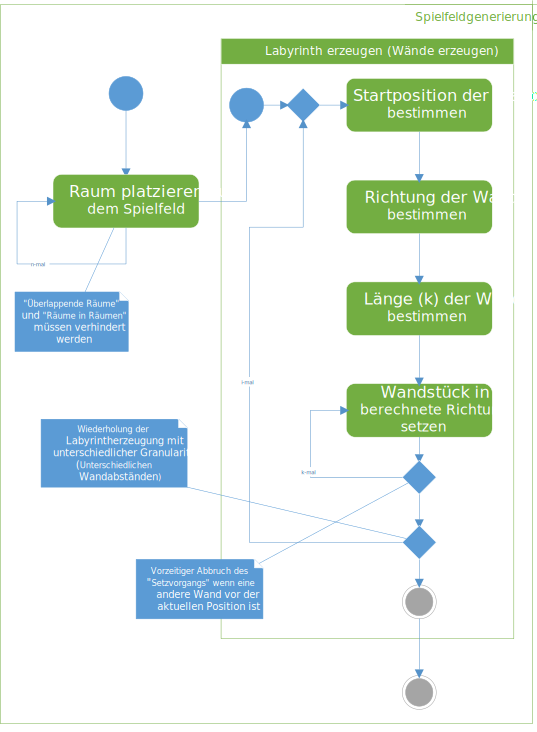
\includegraphics[scale=0.65]{images/spielfeldgenerierung.pdf}

\end{figure}

